\documentclass[11pt, letterpaper]{article} 

%%%% ----- PACKAGES ---- %%%%

% Fonts & Colors
\usepackage[utf8]{inputenc}
\usepackage[T1]{fontenc}
\usepackage{lmodern}
\usepackage[svgnames,usenames,dvipsnames,x11names,table]{xcolor}
\usepackage{microtype}

% Math 
\usepackage{amsmath,amsthm}
\usepackage{amsfonts,eucal,amssymb,amscd,empheq,bm,mathtools}
\usepackage{mathrsfs}
\usepackage{calc} 

% Tikz & boxes
\usepackage{tikz}
\usepackage[framemethod=tikz]{mdframed}
\usepackage{framed}

% interface for floats (Figures/Tables), allows 'H' option
\usepackage{float}

% expanded footnote package
\usepackage{bigfoot}

% refinements 
\usepackage{setspace}
\usepackage{graphicx}
\usepackage[normalem]{ulem}
\usepackage{fancyhdr}
\usepackage[pdftex]{hyperref}
\usepackage{url}

%\usepackage{amsmath, amsfonts, amsthm}
%\usepackage[svgnames,table]{xcolor}
\usepackage[hang, small, labelfont=bf, up, textfont=it]{caption}
\usepackage{booktabs} 

\usepackage{enumerate}
\usepackage{listings}
\usepackage{marginnote}
\usepackage{mparhack}

\usepackage{longtable}
\usepackage[labelfont=bf,indention=0cm]{caption}
\usepackage{subcaption}

\usepackage{verbatim}
\usepackage[makeroom]{cancel}

\usepackage{geometry}
\usepackage[most]{tcolorbox}
\usepackage{tabularx}

\usepackage{bookmark}
\usepackage[lite]{amsrefs}
\usepackage{arydshln}

\usepackage{booktabs}
\newcounter{lecnum}
\usepackage{nicefrac}
\usepackage{tcolorbox}
\tcbuselibrary{theorems}

\usepackage{enumitem} 
\setlist{noitemsep} 
\usepackage{sectsty} 
\allsectionsfont{\usefont{OT1}{phv}{b}{n}}

\makeatletter
\def\@seccntformat#1{\csname the#1\endcsname.\quad}
\makeatother

\usepackage{geometry}
\geometry{
	top=0.75in,
	bottom=0.75in,
	left=1.5in,
	right=1.5in,
	includehead,
	includefoot,
	%showframe, 
}

\hypersetup{pdftex, colorlinks, citecolor=blue, filecolor=blue, linkcolor=blue, urlcolor=blue}

\pagestyle{fancy}
\PassOptionsToPackage{normalem}{ulem}
\makeindex
\setlength{\headheight}{12pt}


\setlength{\columnsep}{7mm} % Column separation width
\usepackage[T1]{fontenc}
\usepackage[utf8]{inputenc} 
\usepackage{XCharter} 
\usepackage{fancyhdr} 
\pagestyle{fancy} 

\renewcommand{\headrulewidth}{0.0pt} 
\renewcommand{\footrulewidth}{0.0pt}

%\renewcommand{\footnotesize}{\scriptsize}
\setlength{\skip\footins}{10pt}

\usepackage[numbered,framed]{matlab-prettifier}
\lstset{style= Matlab-editor,
    basicstyle = \mlttfamily\footnotesize,
    breaklines=false,
    %backgroundcolor=\color{light-gray},
    numbersep=5pt,
    xleftmargin=.25in,
    xrightmargin=.25in 
} 

%\usepackage[parfill]{parskip}
%\setlength{\parskip}{4pt} 
\setlength{\parindent}{0pt}

% format/layout adjustments
\newcommand{\n}{\vskip 6pt \noindent}
\newcommand{\nn}{\vspace{8mm} \noindent}
\newcommand{\ns}{\vspace{8mm}}

% for adjustwidth environment
\usepackage[strict]{changepage}

% environment derived from framed.sty: see leftbar environment definition
\definecolor{formalshade}{rgb}{0.95,0.95,1}
\definecolor{darkBlue}{RGB}{25,25,112}

\newenvironment{formal}{%
\small
  \def\FrameCommand{%
    \hspace{1pt}%
    {\color{darkBlue}\vrule width 2pt}%
    {\color{formalshade}\vrule width 4pt}%
    \colorbox{formalshade}%
  }%
  \MakeFramed{\advance\hsize-\width\FrameRestore}%
  \noindent\hspace{-4.55pt}% disable indenting first paragraph
  \begin{adjustwidth}{}{7pt}%
  \vspace{-12pt}
  \vspace{2pt}\vspace{2pt}%
}
{%
  \vspace{2pt}\end{adjustwidth}\endMakeFramed%
}

\usepackage{sectsty}
\subsectionfont{\normalfont\itshape}


% Removes the section number from the header when \leftmark is used
\renewcommand{\sectionmark}[1]{\markboth{#1}{}} 

\usepackage{titlesec}
\titleformat{\subsubsection}{}{\thesubsubsection}{1em}{\itshape}



%\nouppercase\leftmark % Add this to one of the lines below if you want a section title in the header/footer

% Headers/ footers
\lhead{}
\chead{} 
\rhead{}

\lfoot{} 
\cfoot{} 
\rfoot{} % Right footer, "Page 1 of 2"

\fancyfoot[C]{\fontsize{9}{12} \selectfont \vspace{12pt} \textit{\footnotesize{\thepage}}}

% Page style for the first page with the title
\fancypagestyle{firstpage}{ 
	\fancyhf{}
	\renewcommand{\footrulewidth}{0pt}
}

%----------------------------------------------------------------------------------------
%	TITLE SECTION
%----------------------------------------------------------------------------------------

\newcommand{\authorstyle}[1]{{\large\usefont{OT1}{phv}{b}{n}\color{DarkRed}#1}} 
\newcommand{\institution}[1]{{\footnotesize\usefont{OT1}{phv}{m}{sl}\color{Black}#1}}
\usepackage{titling} 
\newcommand{\HorRule}{\noindent \color{DarkGoldenrod}\rule{\linewidth}{0pt}} 

\pretitle{
\centering
	\vspace{-5pt} 
	\HorRule\vspace{10pt} 
	\fontsize{24}{28}\usefont{OT1}{phv}{m}{n}\selectfont 
	\color{DarkRed} 
}
\posttitle{
\centering
\par\vskip2pt
} 

\preauthor{} 
\postauthor{ 
	\vspace{0pt} 
	\par\HorRule
	%\vspace{20pt} 
	\vspace{-1cm} 
}


\theoremstyle{break}
\newtheorem{example}{Example}[section]

\mdfdefinestyle{mystyle}{
  hidealllines=true,
  leftline=true,
  innerleftmargin=10pt,
  innerrightmargin=10pt,
  innertopmargin=10pt,
}


\newmdtheoremenv[style=mystyle]{example2}{Example}




\theoremstyle{definition}
\newtheorem{defnn}{Definition}
\newtheorem*{tst*}{}
\newmdtheoremenv[style=mystyle]{defnn2}{Definition}

\newtheorem*{Alg*}{Algorithm}
\newtheorem*{rmk*}{Remark}
\newtheorem*{thm}{Theorem}
\newcommand{\Recall}{\vspace{4mm}\noindent \bd{\ul{Recall}}}
\newcommand{\Note}{\vspace{4mm}\noindent \bd{\ul{Note}}}
\newcommand{\Question}{\vspace{4mm}\noindent \bd{\ul{Question}}}

\newcommand{\Problem}[1]{\vspace{4mm}\noindent {\large\bd{\ul{Problem #1}}}}



		%%%%%%%%%%%%%%%%%%%%%%%%%%%%%%%% DEFINITIONS  %%%%%%%%%%%%%%%%%%%%%%%%%%%%%%%%%%%

\theoremstyle{definition}
\newtheorem{quest}{Question Set:}
\newtheorem{deliv}{Deliverable}



%%%%%%      MATH ENVIRONMENT      %%%%%%%%

% align
\newcommand{\eq}[1]{\begin{align*}#1\end{align*}}

% tags
\newcommand{\tagit}[1]{\tag{\it{#1}}}
\newcommand{\tagitb}[1]{\textcolor{blue}{\tag{\it{#1}}}}



% font
\newcommand{\ul}[1]{\underline{#1}}
\renewcommand{\it}[1]{\textit{#1}}
\newcommand{\bd}[1]{\textbf{#1}}
\newcommand{\bul}[1]{\textbf{\ul{#1}}}
\newcommand{\bit}[1]{\textbf{\textit{#1}}}



% shortcuts for letters, symbols & etc
\def\nhat{\bm{\hat{n}}}

\newcommand{\Z}{{\mathbb{Z}}}
\newcommand{\R}{{\mathbb{R}}}
\newcommand{\N}{{\mathbb{N}}}
\newcommand{\F}{{\mathcal{F}}}
\newcommand{\C}{{\mathcal{C}}}
\newcommand{\W}{{\mathcal{W}}}
\newcommand{\E}{{\mathcal{E}}}
\newcommand{\A}{{\mathcal{A}}}
\newcommand{\X}{{\mathbb{X}}}


% colors
\colorlet{shadecolor}{Red!5}
\colorlet{framecolor}{Red!1}
\definecolor{dkred}{RGB}{165,0,0}

%%%%% BOXED EQUATIONS %%%%%%%
\newcommand*\widefbox[1]{\fbox{\hspace{2em}#1\hspace{2em}}}

% shading
\newenvironment{frshaded}{
 \def\FrameCommand{\fboxrule=\FrameRule\fboxsep=\FrameSep \fcolorbox{framecolor}{shadecolor}}%
 \MakeFramed{\FrameRestore}}%
 {\endMakeFramed}

 \newenvironment{frshaded*}{%
 \def\FrameCommand{\fboxrule=\FrameRule\fboxsep=2\FrameSep \fcolorbox{framecolor}{shadecolor}}%
 \MakeFramed{\advance \hsize - \width \FrameRestore}}%
  {\endMakeFramed}



% horizontal & vertical lines
\newcommand*{\vertbar}{\rule[-1ex]{0.5pt}{2.5ex}}
\newcommand*{\horzbar}{\rule[.5ex]{3ex}{0.5pt}}

%%%%%%      SHORTCUTS     %%%%%%%%
\newcommand{\dt}{{\Delta t}}
\newcommand{\dx}{{\Delta x}}
\newcommand{\idt}{{\frac{1}{\Delta t}}}
\newcommand{\idx}{{\frac{1}{\Delta x}}}
\newcommand{\dtdx}{\frac{\Delta t}{\Delta x}}
\newcommand{\dxdt}{\frac{\Delta x}{\Delta t}}

\newcommand{\Qin}{{Q_{i}^{n} }}
\newcommand{\Qini}{{Q_{i}^{n \+ 1} }}
\newcommand{\Qimi}{{Q_{i}^{n \- 1} }}
\newcommand{\Qinp}[1]{{Q_{i}^{n \+ #1} }}

\newcommand{\qx}{q_{,x}}
\newcommand{\qxx}{q_{,x,x}}
\newcommand{\qt}{q_{,t}}
\newcommand{\qtt}{q_{,t,t}}

\newcommand{\ordii}{\ord( \dx^2)}
\newcommand{\ordiii}{\ord( \dx^3)}

\renewcommand{\uplus}{u^{\+}}
\newcommand{\uminus}{u^{\-}}

\newcommand{\Fii}[2]{\F_{ i \+ \h}^{n \+ \h}}
\newcommand{\Fnn}[2]{\F_{ #1}^{#2}}
\newcommand{\FF}{\Scale[1.4]{\mathscr{F}}}

\newcommand{\sumN}{\sum_{i \= 1}^{N} }
\newcommand{\summ}{\sum_{p \= 1}^{m} }
\newcommand{\suminf}{\sum_{i \= -\infty}^{\infty} }

\newcommand{\ord}{{\mathcal{O}}}
\newcommand{\into}{\rightarrow}

\newcommand{\stari}{\raisebox{.2\height}{\scalebox{0.9}{\ensuremath{\hspace{0.25mm} \star}}}}


\newcommand{\lp}{\lambda^{(p)}}

%% SUPERSCRIPTS
\newcommand{\soln}{\it{sol}\textsuperscript{\ul{\it{n}}}}
\newcommand{\Soln}{\it{Sol}\textsuperscript{\ul{\it{n}}}}
\newcommand{\eqn}{\it{eq}\textsuperscript{\ul{\it{n}}}}
\newcommand{\Eqn}{\it{Eq}\textsuperscript{\ul{\it{n}}}}

\newcommand{\st}{\textsuperscript{\ul{\it{st}}} }
\newcommand{\nd}{\textsuperscript{\ul{\it{nd}}} }

% create a matrix: use &, \\ as normal
\newcommand{\mtx}[1]{\left(\begin{matrix}#1\end{matrix}\right)}


%%%%% EQUATIONS  %%%%%%

\newcommand{\burgers}{\eq{  q_{,t} + \Big( \h q^2 \Big)_{,x} = 0 }} 			% Burger's Eqn






%%%%% GRAPHICS %%%%%
\newcommand{\gfxi}[1]{
\vspace{3mm}
  \begin{center}
    \begin{figure}[h!]
    \includegraphics[height=45mm]{#1}
    \end{figure}
  \end{center}
}

\newcommand{\gfxii}[2]{
\vspace{3mm}
  \begin{center}
    \begin{figure}[h!]
    \includegraphics[height=#1mm]{#2}
    \end{figure}
  \end{center}
}

% figure + equation/text, side by side
\newcommand{\gfxss}[2]{
\vspace{3mm}
\noindent\begin{minipage}{.45\textwidth}
 	\centering
   		\includegraphics[height=45mm]{#1}
  		\label{fig:figure}
\end{minipage}
\begin{minipage}{.45\textwidth}
#2
\end{minipage}
}

 
\graphicspath{{./gfx/}}

\definecolor{light-gray}{gray}{0.98}
\usepackage[bottom,hang,flushmargin]{footmisc}
\renewcommand{\footnotesize}{\scriptsize}

\usepackage{siunitx}

\title{ \textsc{Lab 0: \\ Matlab Tutorial} \\ {\large  \color{darkgray} ME 436 Heat Transfer - Fall 2017}}

\begin{document}
\date{}
\maketitle
\thispagestyle{firstpage} 


\section*{Introduction}

This short tutorial is designed to familiarize you with \texttt{MATLAB} and the general structure of the homework assignments to come. Be sure to read through this document carefully and check out the resources section at the end. Finally, if you have any questions or difficulties, be sure to contact your TA as soon as you can.

\subsection*{Scope}

The purpose of each homework assignment is to save \textit{you} time. Once completed, you will have a plug-and-play mathematical model ready to go. 
As some of you may be aware, this is a slight departure from previous labs, in which much of the analysis is generally performed after data collection. 
By shifting some of the weight from \textit{post-processing} onto the \textit{pre-lab}, this frees up precious lab time and provides a more balanced workload for everyone. 
More importantly, this approach allows us to dive deeper into the experiments and ultimately ask more interesting questions.

\n
So, rather than having each group build an Excel sheet from scratch to analyze your collected data (at home, after the lab), we will provide you with a set of partially completed \texttt{MATLAB} scripts and sample data.
Then, your homework assignment (individual) will be to complete these \texttt{MATLAB} scripts and answer a few short questions. To receive full credit, you must submit your responses at the \textit{beginning} of your lab period. 
You will then use these mathematical models in-class to quickly process your experimental data.
 
\subsection*{Why Matlab?}

From our experience, far too much time is lost slogging through the minutiae -- rather than focusing on the more critical aspects. With the assistance of \texttt{MATLAB}, we can essentially sidestep many of these uninspiring -- and often mundane -- tasks that detract from the core laboratory objectives. For example, with Excel, locating cell numbers, debugging, formatting charts, and performing repetitive calculations \textit{(property look-up's, interpolation, unit conversions \&, etc.)}, can be very mundane... Taken together, these tasks can quickly snowball into a much larger (and time-consuming!) task than initially anticipated. More importantly, however, these mundane details dilute the overall take-away message. We should be more focused on performing experiments and exploring data - rather than fighting with computer software. That being said...


\subsection*{Not a Matlab fan?}

No problem. This isn't a \texttt{MATLAB} course --  nor is it an Excel course -- we're interested in Heat Transfer.  Thus, we only expect the \textit{bare minimum} on the programming front. Anything beyond entry-level will be explicitly provided to you.

\section*{Getting Started}
As stated above, this short tutorial is designed to help familiarize you with the basic format of the homework assignments. In addition, this document has been written to provide a comprehensive explanation at each step along the way. You may want to use this as a reference throughout the semester. In general, the assignment instructions will be written more concisely. 

\n
First, you will always need to download the starter code from Blackboard (Bb), and \textit{extract} (unzip) its contents to the directory in which you wish to complete the exercise\footnote{\textit{Note: when using the Heat Transfer Lab computers, you \ul{must} extract your code to the local hard drive: \texttt{C:/temp/}, NOT to the server (ie., Desktop, Group Folder, \&, etc.) See additional details at the end of this document.}}. Before attempting, make sure that you have completed all of the \textit{prerequisites} below.


\section*{Prerequisites}
Generally, in this section you will find a short list of the essentials that should be completed \textit{before} attempting the assignment. For \textit{example}, in Lab 1 you will see:
{\small
\begin{itemize}
    \item Review the \bit{textbook sections:} 2.1, 2.2 \& 3.1-3.1.4,
    \item Review the \bit{experiment procedures}, 
    \item Watch the \bit{pre-lab videos} on Blackboard (Bb), and
    \item Complete the \bit{pre-lab quiz} on Bb.
\end{itemize}
}


\subsection*{Files included in this exercise:}
Now we are ready to start the assignment. Once you have unzipped the contents of the starter package, you should have the following files and folders:

\begin{itemize}
\renewcommand\labelitemi{-- }
   \item \texttt{ex0.m} - \it{main file that you will work out of.}
    \item \texttt{/lib} - \it{functions and files that work behind the scenes. It's best not to touch them.}
\renewcommand\labelitemi{[$\star$]}
    \item \texttt{plotData.m} - \it{function that plots your data - you \ul{will} need to adjust this one.}
\end{itemize}

\noindent
$\star$ indicates files that you will need to complete.\\

In general, you will be using the script titled \texttt{ex<lab no>.m}, without making any sensible changes to it. However, sometimes you will be required to comment out the \texttt{return} commands at the end of each section, to better understand each step of the analysis. More information about this will be provided below.

\setcounter{section}{-1}
\section{Warm-Up \& System Check}

Before starting, it is often useful to understand the data by first visualizing it. In particular, for the upcoming experiment (Lab 1), we need to make sure that our collected data is at steady--state. Hence, for this first tutorial, we will load a sample dataset and then plot it using \texttt{MATLAB}. In the process, we will also make sure that our system is setup correctly.

\subsection{Load Data}
Now, make sure that you have \texttt{MATLAB} started and the script titled \texttt{`ex0.m'} opened up in the editor. If you have any troubles with this step, be sure to check out the resources at the end of this document or ask your TA.

\n
Now, with \texttt{ex0.m} open, the first thing you will see is the \textit{Documentation Header:}

\n
\begin{lstlisting}[numbers=none]
%% ME 436L Heat Transfer
% Lab 0 | MATLAB Tutorial
%
%  INSTRUCTIONS
%  ------------
%
%  This file contains code that will guide you through the assignment. Be 
%  sure to follow the instructions provided in the attached document.
%
%  NOTE: You will need to complete the following functions:
%
%       plotData.m
%
% For this exercise, you will be required to comment out the 'return'
% command line at the end of each section, to ensure that you fully
% understand each step of the analysis.
%%
% Written By: Spencer Pfeifer | Revision: Paola G. Pittoni
% Date:   8/24/17
%
%#ok<*UNRCH>
\end{lstlisting}
\n
This provides information as to what the script does, who wrote it, and when. Now, skipping the \textit{Initialization} section, we get to a section titled \textit{`Load Data'}. Here, we load a sample dataset from a text file and store it into the variable \texttt{M}:
\n
\begin{lstlisting}[numbers=none]
% load tab separated data
M = load('data.txt'); 
\end{lstlisting}
\n

Once you have pressed `Run,' you will now have a matrix $M$ of size $93 \times 11$ ($rows \times columns$), or $M \in \mathbb{R}^{93 \times 11}$. The columns in $M$ are defined as follows:
\\
{\small
\begin{center}\renewcommand{\arraystretch}{1.5}
\begin{tabular}{|c | c | c | c | c | c | c |}
\hline
\rowcolor{light-gray}
    1 & 2 & 3 & \dots & 9 & 10 & 11 \\ 
    \hline
   \cellcolor{green!10} $time (s)$ & \cellcolor{red!10}$TC_1$ & \cellcolor{red!10}$TC_2$ & \cellcolor{red!10}$\dots$ & \cellcolor{red!10}$TC_8$ & \cellcolor{orange!10}$Voltage, V$ & \cellcolor{orange!10}$Current, A$ \\ 
\hline
\end{tabular}
\end{center}
}

In which $TC_n$ refers to the thermocouple number, read in degrees Celsius. Next, you will see a line that looks similar to the following:
\n
\begin{lstlisting}[numbers=none]
% COMMENT ME OUT!!
break_msg; dbstack; return;
\end{lstlisting}

\n
This is what we refer to as a \texttt{return} command. In short, this line will exit the program and leave you with a message that looks similar to the following:
\begin{figure}[H]
    \begin{center}
        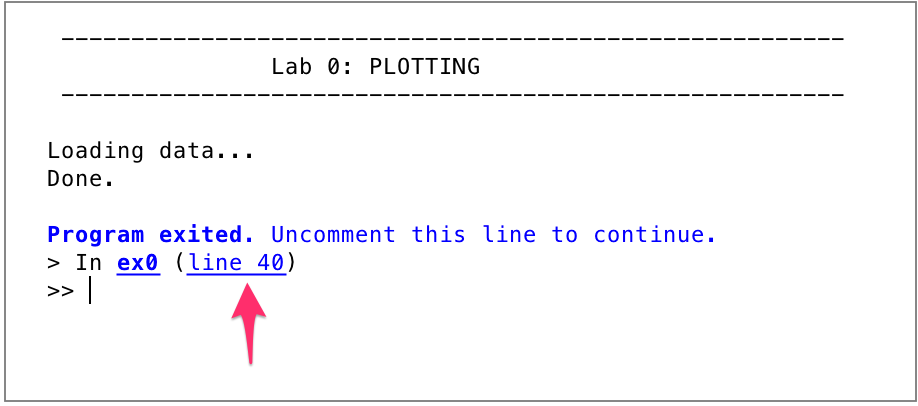
\includegraphics[width=90mm]{gfx/program_exit_line.png}
    \caption{Sample Matlab Output. \textit{Tip: You can click on the line number and it will take you to the exact line of the \texttt{return} function.}}
    \end{center}
\end{figure}
\vspace{-2mm}
You will need to \textit{comment out} this line (place a \% out front) in order to continue.

\subsection{Extract \& Plot Data}
Next, let's separate out this data into more meaningful variables.\footnote{\textit{Note: if you are not familiar with the syntax, check out: \href{https://www.mathworks.com/company/newsletters/articles/matrix-indexing-in-matlab.html}{Matrix indexing in Matlab}  }} 
\n
\begin{lstlisting}[numbers=none]
t = M(:,1);         % get time vector, [s]
dat = M(:,2:9);     % get temps, [C]
V = M(:,10);        % Voltage, [V]
I = M(:,11);        % Current, [A]
\end{lstlisting}

\n
You should take this moment to press \texttt{Run} and open the \it{workspace} to confirm the above variable assignments. Now, after removing the \texttt{return} command, let's plot our temperatures with time by executing the following lines:

\n
\begin{minipage}{\linewidth}
\begin{lstlisting}[numbers=none]
figure;         % open new figure
h = plot(dat);  % plot the data
set(h, 'LineStyle', '-', 'LineWidth', 2)   % make sure the lines are readable
\end{lstlisting}
\end{minipage}

\n
\begin{minipage}{\linewidth}
\begin{lstlisting}[numbers=none]
% don't forget to add labels!!
xlabel('Time [s]');
ylabel('Temperature [C]');
title('Transient Data, T/C','FontSize',16);
grid on
\end{lstlisting}
\end{minipage}

\n
Now, if everything was done correctly, you should obtain the Fig.~\ref{fig1} below.
\begin{figure}[H]
    \begin{center}
        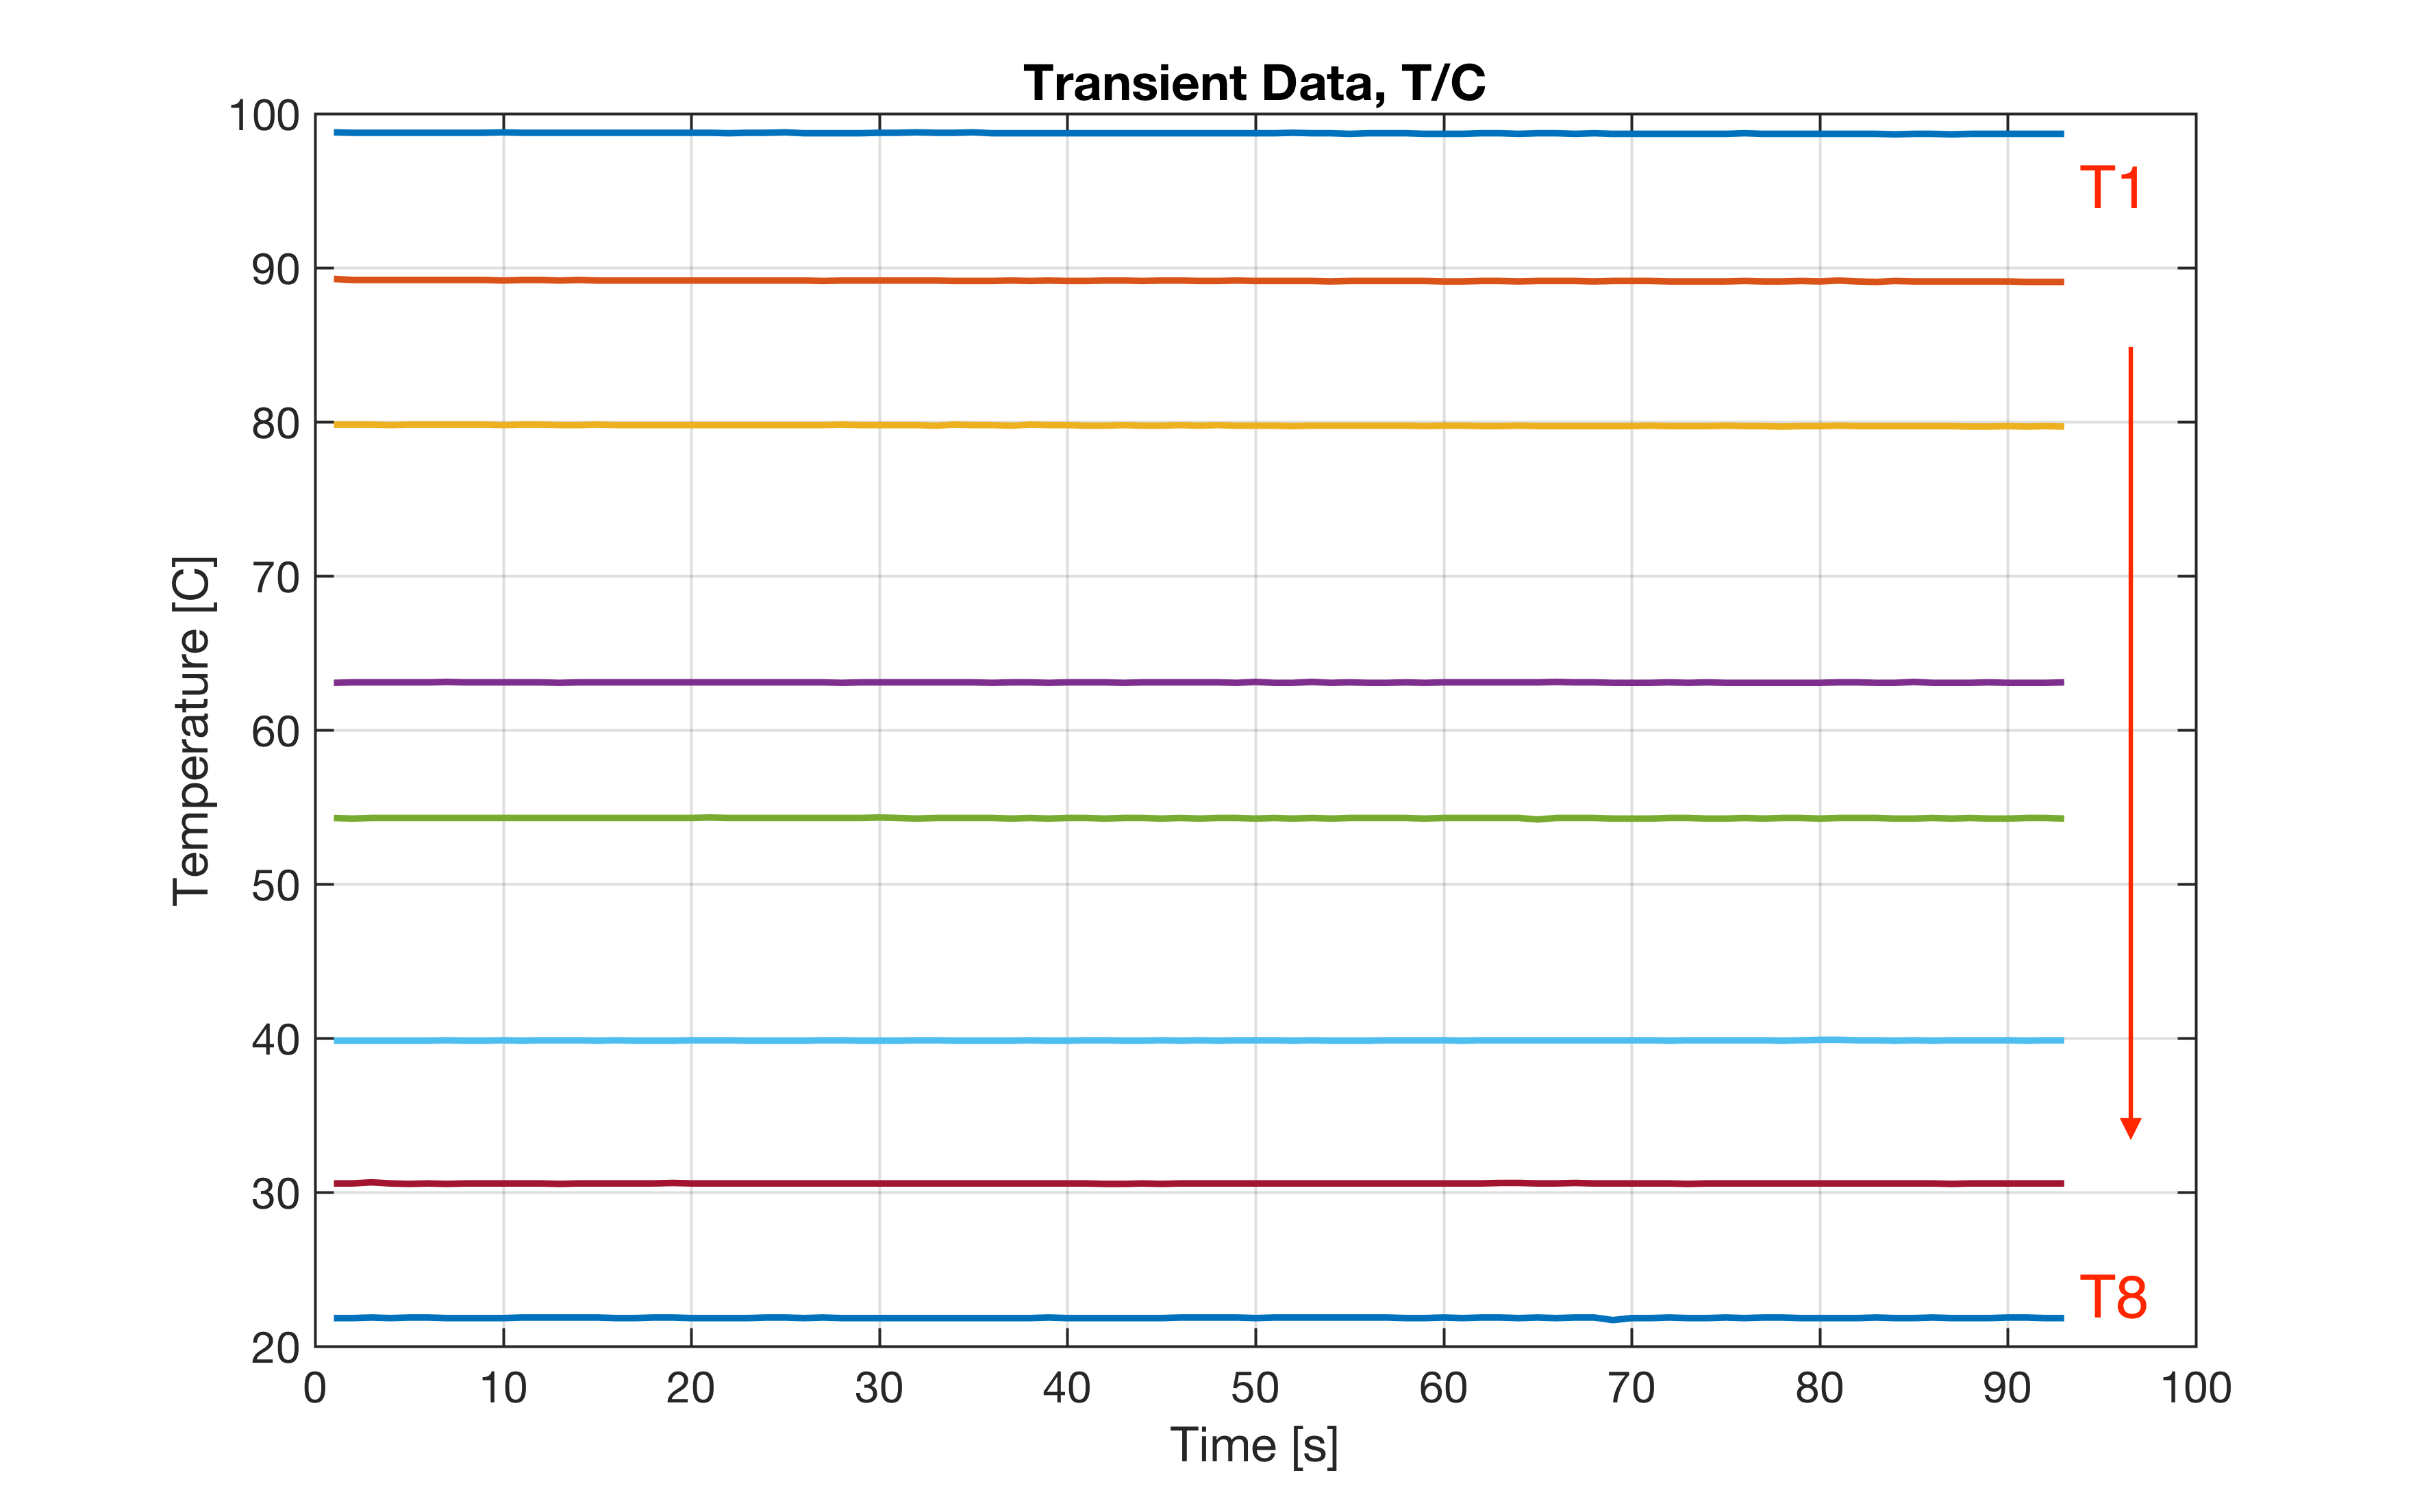
\includegraphics[width=125mm]{gfx/fig1.png}
    \caption{Transient temperature data}\label{fig1}
    \end{center}
\end{figure}

A few quick questions to ask:

\begin{formal}
\begin{quest} \bit{Sanity Check.}
\begin{itemize}
    \item Does your plot match Fig.~\ref{fig1}? 
    \item Is all of our data at steady-state?
\end{itemize}
\end{quest}
\end{formal}

\begin{itemize}
    \item \textit{Note: This blue box will be used to denote your deliverables for the assignment. Be sure to pay close attention.}
\end{itemize}


\begin{center}
\begin{tcolorbox}[enhanced, width=14cm, size=tight, top=-2mm, colback=red!5, colframe=black!50!white, boxrule=0.25pt, boxsep=2mm]
\n
{\small
\bit{Checkpoint} - If you had any difficulties obtaining Fig.~\ref{fig1}, \bul{stop here} and contact your Lab Instructor. You may run into more troubles ahead.
}
\end{tcolorbox}
\end{center}
\hrule

\section{Plot Steady-State Data}

Now, let's plot the spatial temperature distribution. To do this, we simply average the transient data. This is easily done in \texttt{MATLAB} by the $mean( )$ command:

\begin{lstlisting}[numbers=none]
% take an average of the last (~20) points 
N = 20;
Tm = mean(dat(end-N:end,:));      % [C]
Vm = mean(V(end-N:end));          % [V]
Im = mean(I(end-N:end));          % [A]
\end{lstlisting}

Next, we call a \texttt{plotData.m} function to plot our data. As-it-is, this plot function \textit{\ul{is incorrect}} and will not run properly. Therefore, you will need to open \texttt{plotData.m} and adjust code accordingly in order for it to run properly. The sections that you will need to complete are outlined:

\n
\begin{lstlisting}[numbers=none]
% plot first three T/Cs
plot(x(2:4),y(1:3),'ko-','MarkerSize', 8);

% plot middle two T/Cs
% ====================== YOUR CODE HERE ======================

% plot last three T/Cs
% ====================== YOUR CODE HERE ======================


% set labels & axis limits
% ====================== YOUR CODE HERE ======================
xlabel('');
ylabel('');
\end{lstlisting}

\begin{itemize}
    \item \textit{Note: Pay close attention to the instructions.}
\end{itemize}

When you're finished, you must \bit{go back} to \texttt{ex0.m} before you can press \texttt{Run}. If you attempt to run the function \texttt{plotData.m}, you will receive an error. If your adjustments were correct, and \texttt{ex0.m} was properly executed, you should obtain Fig.~\ref{fig2}.


\begin{figure}[H]
    \begin{center}
        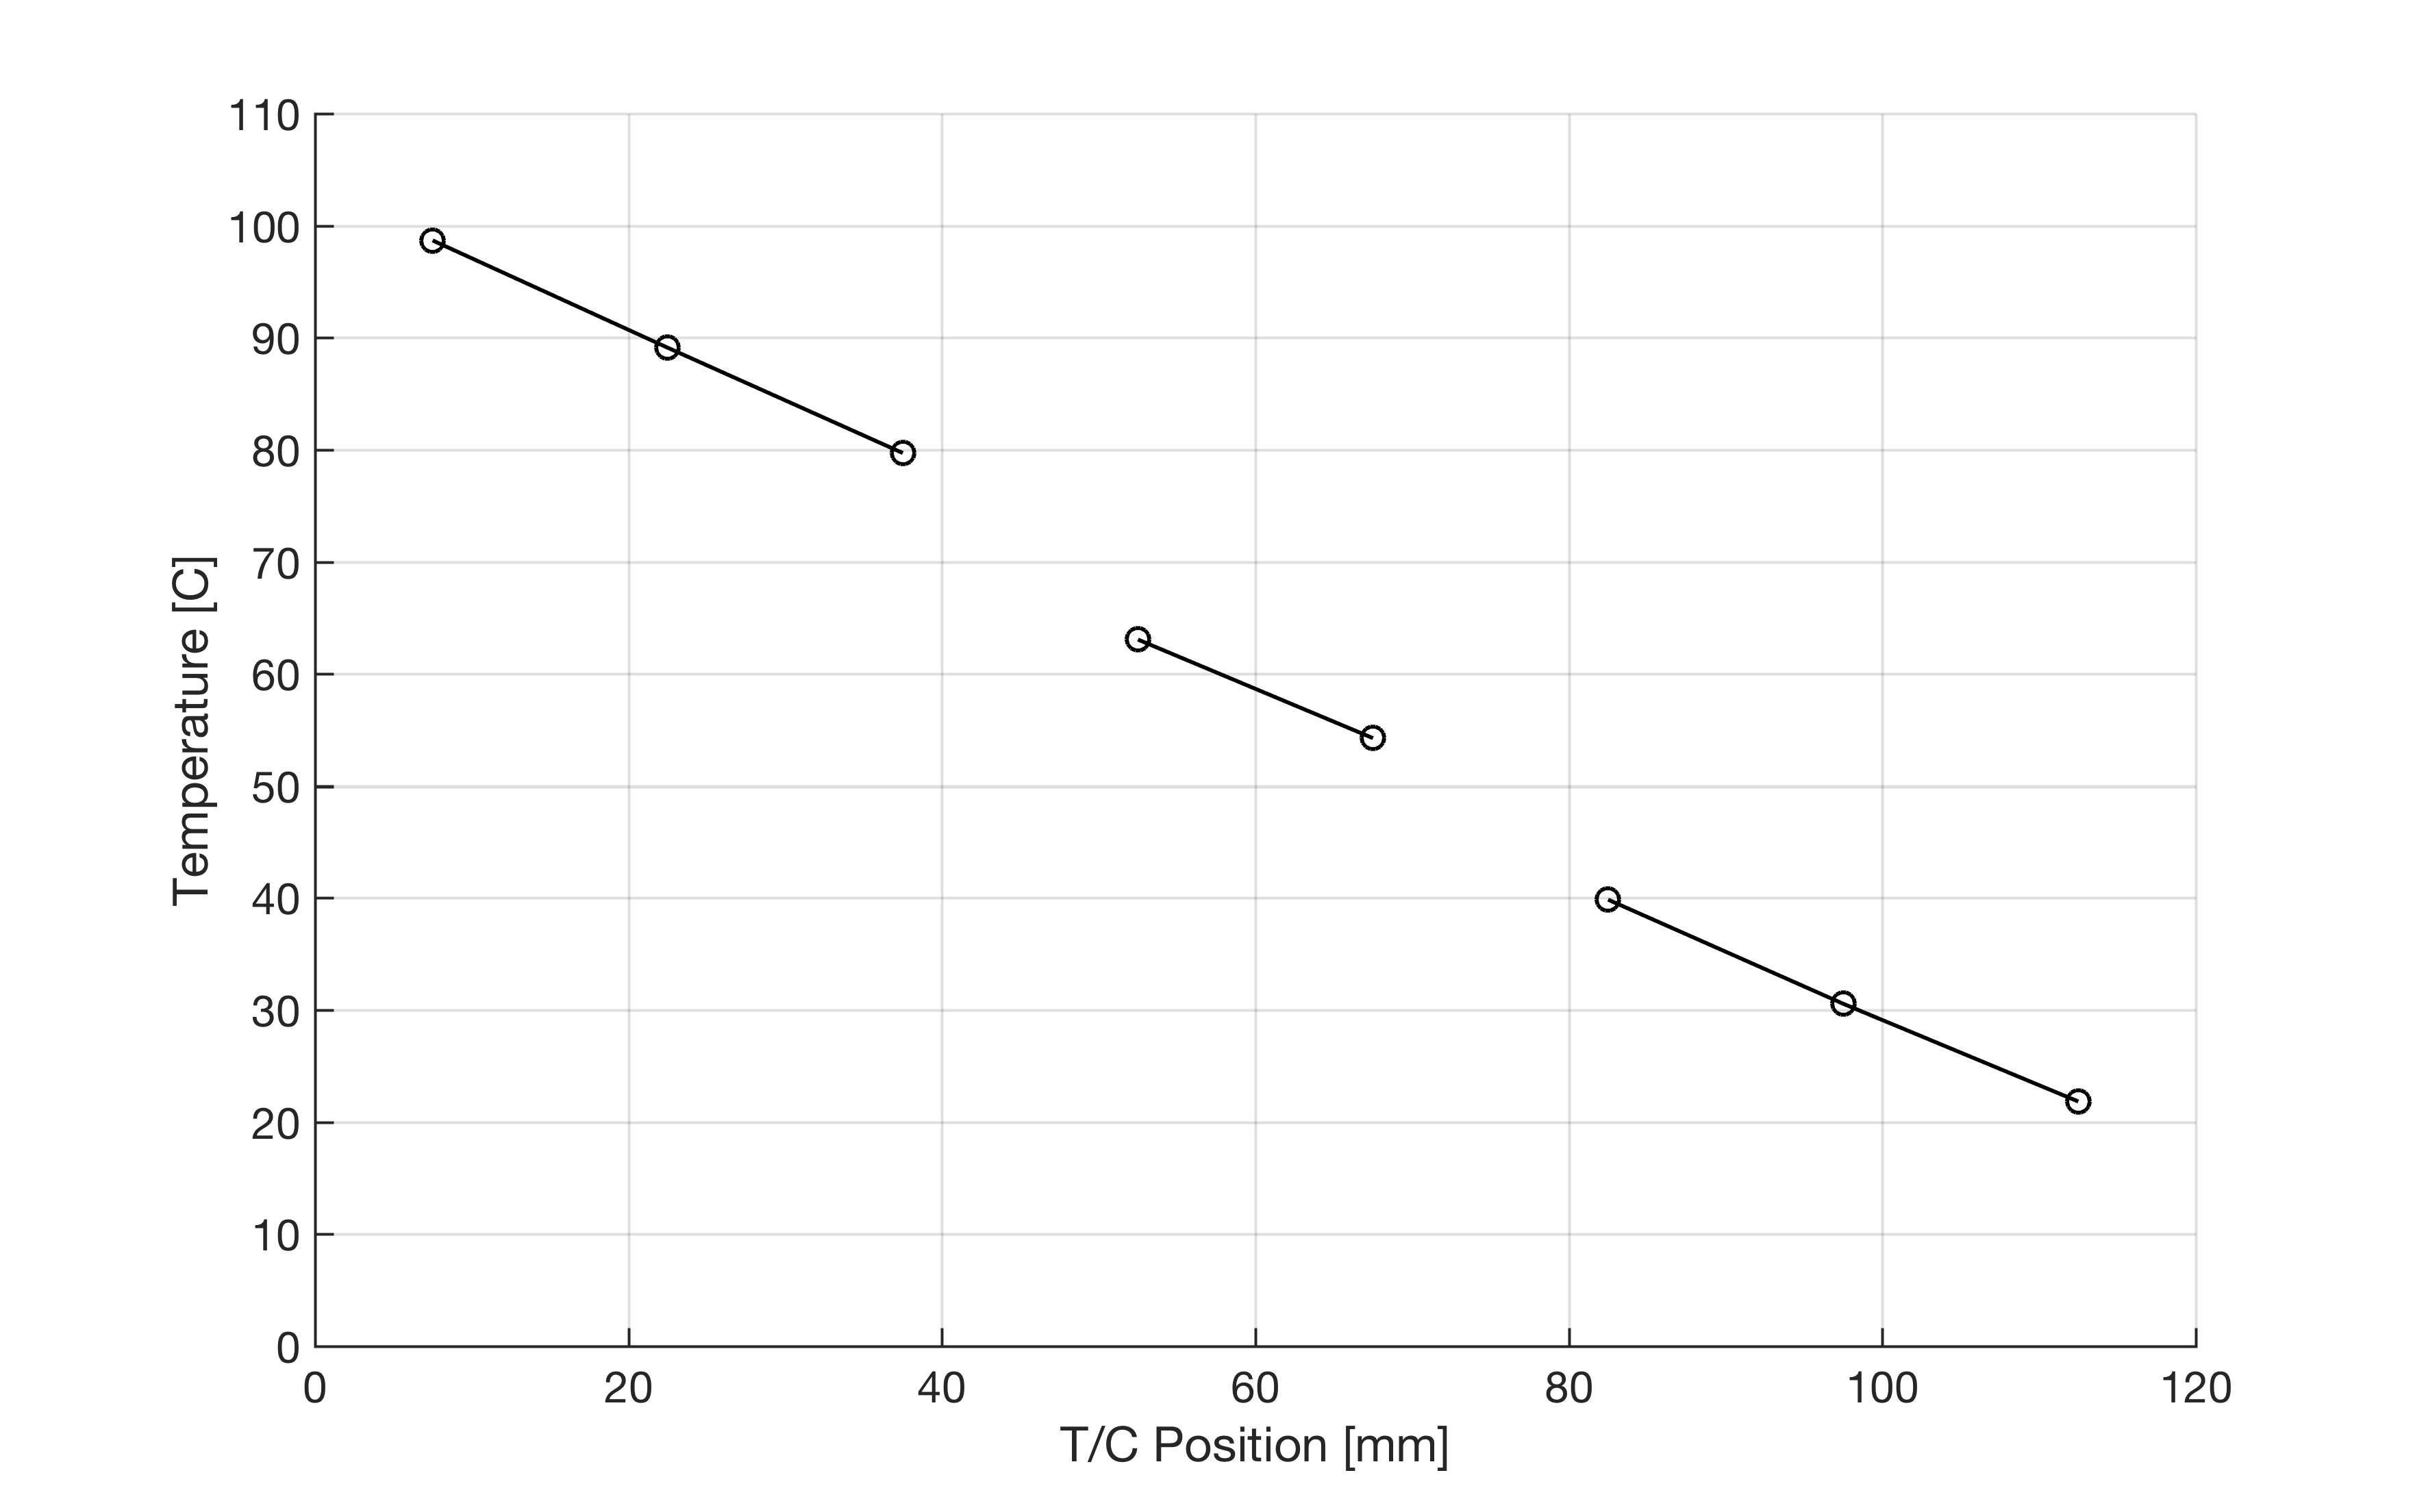
\includegraphics[width=125mm]{gfx/fig2.png}
    \caption{Transient temperature data}\label{fig2}
    \end{center}
\end{figure}

Then, if everything was done correctly above, after commenting out the following \texttt{return} command, you will arrive at a figure that resembles Fig.~\ref{fig3}.

\begin{figure}[H]
    \begin{center}
        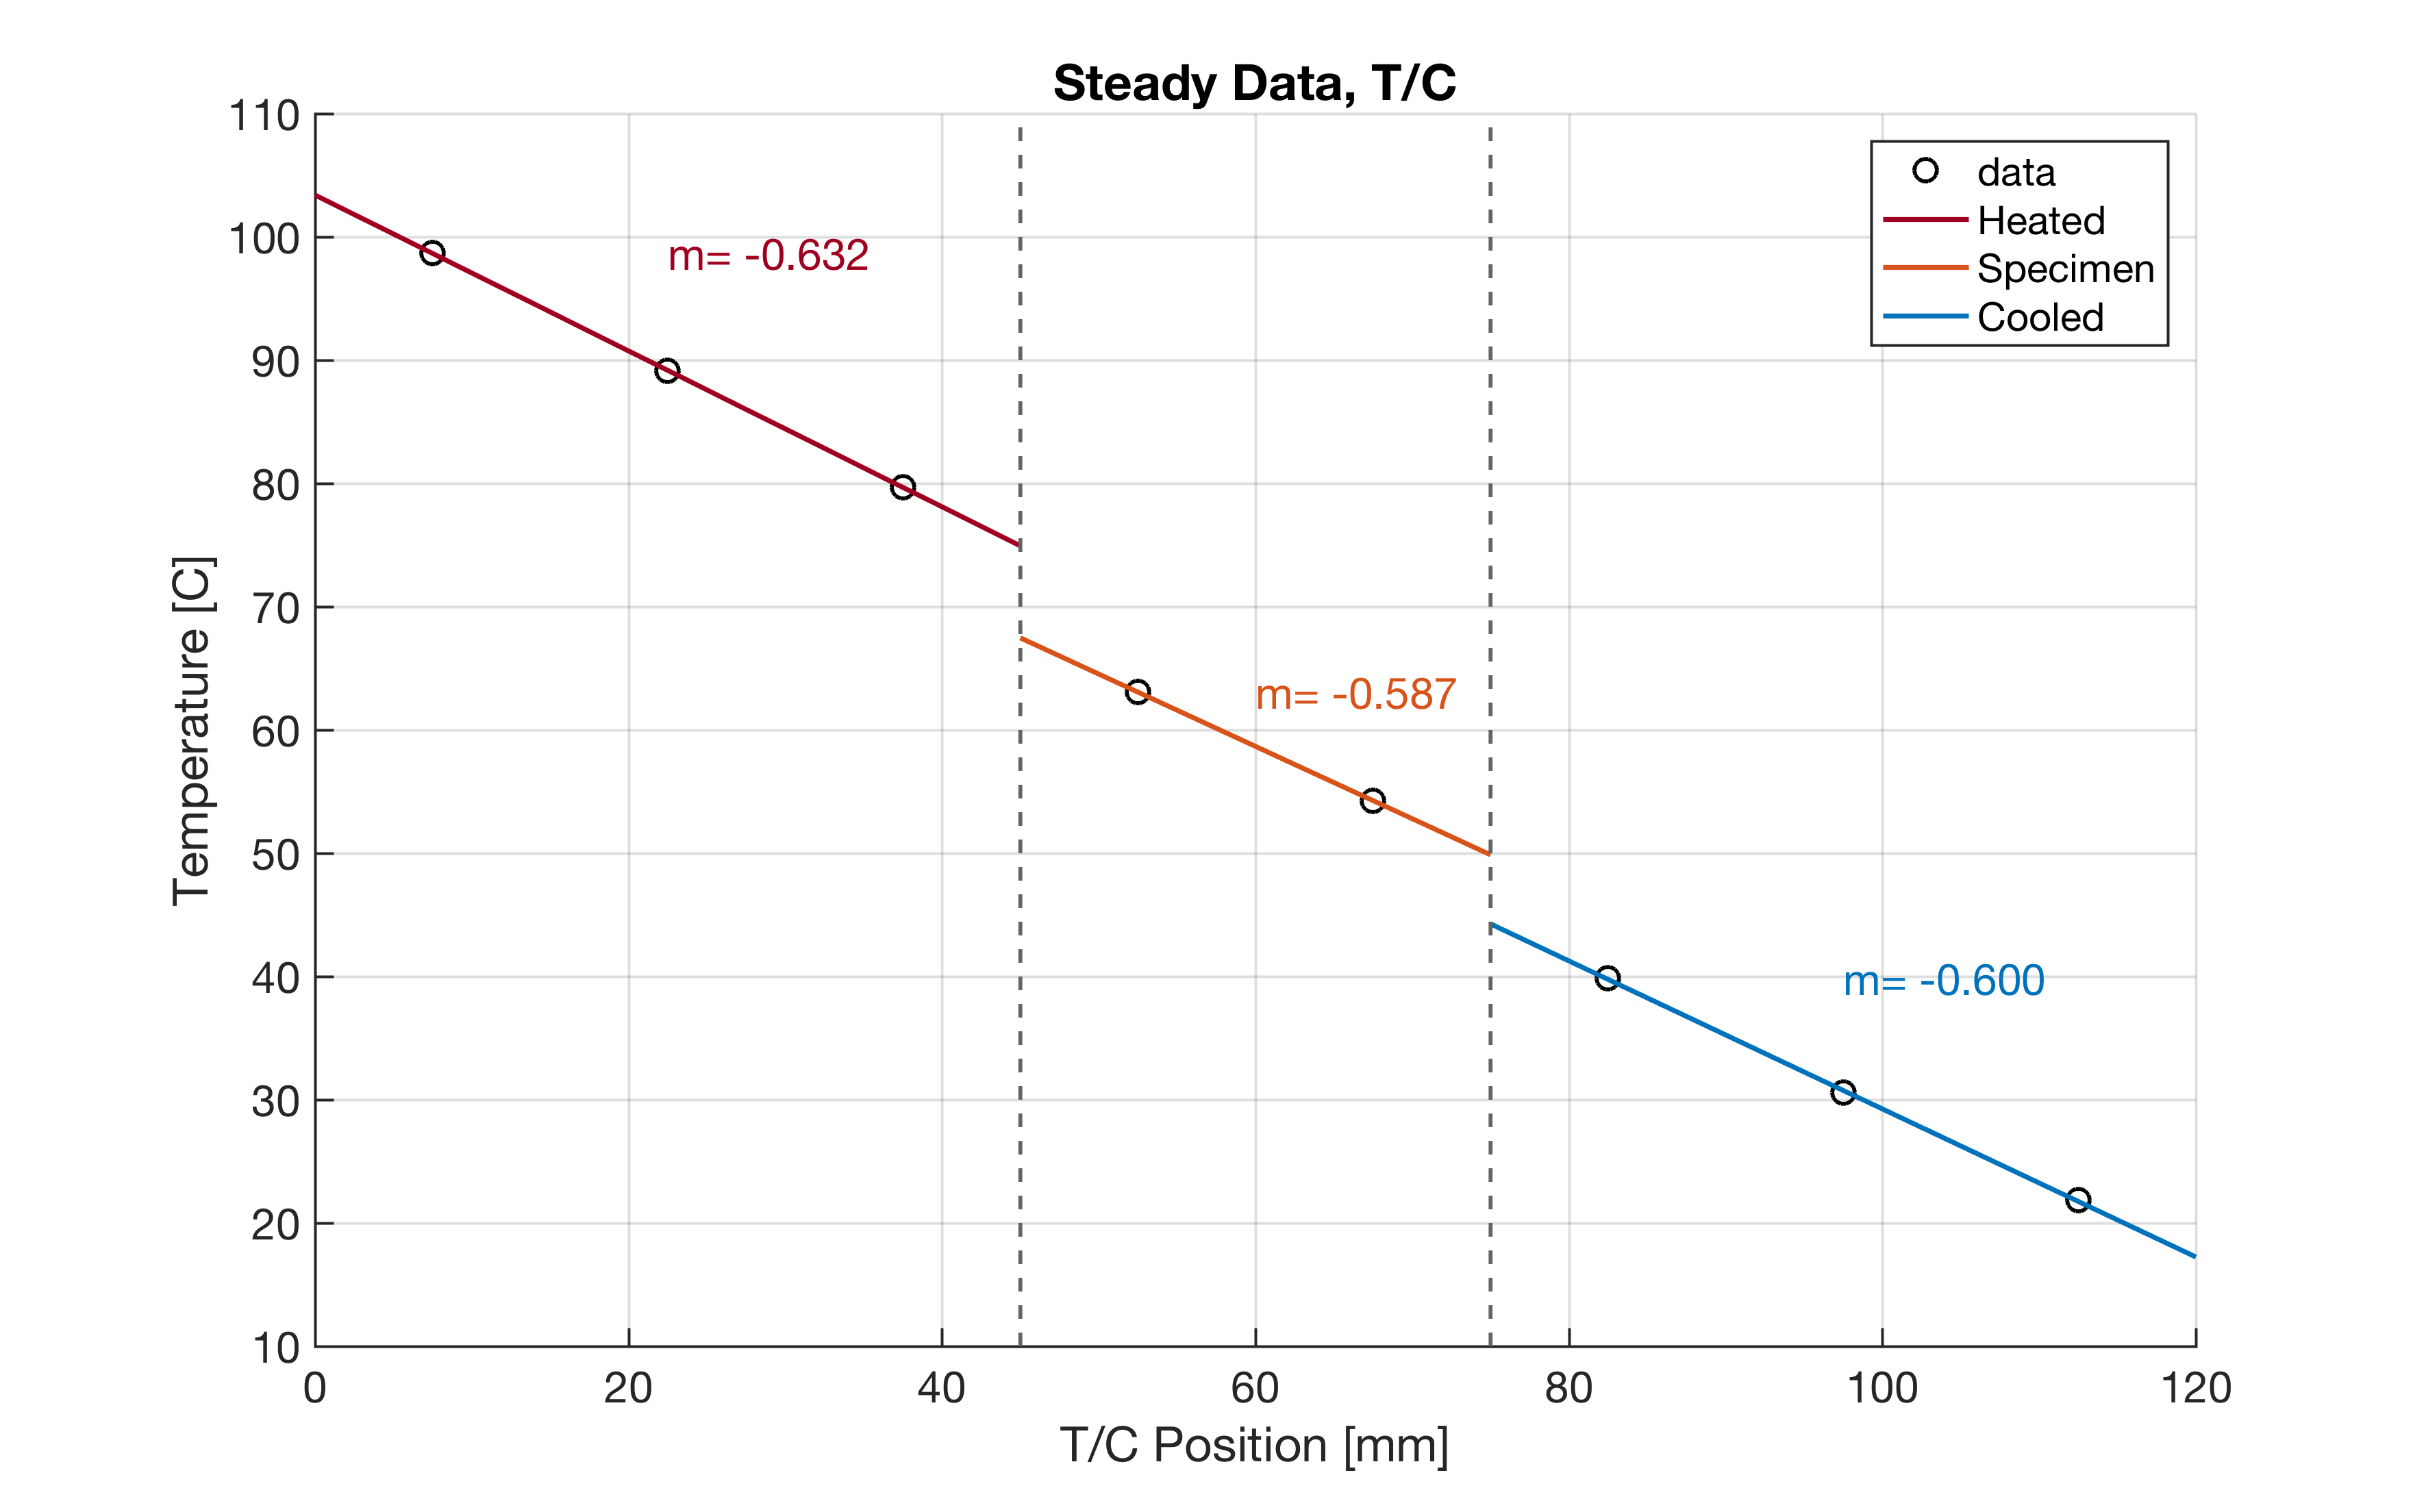
\includegraphics[width=125mm]{gfx/fig3.png}
    \caption{Steady-state T/C data}\label{fig3}
    \end{center}
\end{figure}

Here, we have added regression lines as well as some labels that will make more sense when we get to Lab 1.

\n
The box below outlines the \it{deliverable} for this assignment:

\begin{formal}
    \begin{deliv} \bit{SAMPLE:  Steady-state temperature distribution plot} (Fig.~\ref{fig3}). Export your figure to an image: \texttt{File >> Export Setup (change the properties as desired)>> Export}, and include it in your submission.
    \end{deliv}
\end{formal}

\begin{itemize}
    \item \textit{Note: Do not take a screenshot! Export the figure to a \texttt{.png}.}
\end{itemize}

\section*{Submission}

Generally, once all of the deliverables have been completed, you will simply place the output into a single document, and hand it to your TA at the \textit{beginning} of lab. For this exercise, print Fig.~\ref{fig3} for your 'participation' grade.

\vspace{5mm}
\hrule

\newpage


\section*{Notes:}

\bul{Heat Transfer Lab:}
\begin{itemize}
    

\item \texttt{MATLAB} must be run from the local hard drive: \texttt{C:/temp/}, \bul{NOT} on the server \textit{(ie., \texttt{Desktop}, \texttt{Group Folder}, \&, etc.).} 
    \begin{itemize}
    \setlength\itemsep{0.5em}
         \item \bit{Reason:} This will cause a chain of problems. The server directories are shared across all HT Lab computers, and synchronized every few minutes. 
         \item \textit{\ul{Common scenario:}} Two people unknowingly edit the same document. Once the server synchronizes, one of those two people \bul{will lose all of their work.}
    \end{itemize}

    \item You \textit{\ul{must}} close Matlab when you're done for the day.
    \begin{itemize}
    \setlength\itemsep{0.5em}
         \item \bit{Reason:} The \texttt{addpath(`./lib');} command adds \ul{your} \texttt{./lib} folder to the \texttt{MATLAB} path, while the program remains open. If you do not close Matlab the next section will use \ul{your} data.
    \end{itemize}
    
\end{itemize}

\bul{General:}
\begin{itemize}
    \setlength\itemsep{0.5em}
    \item \textit{\ul{Do not rename any functions!}} These are name (and case) sensitive. If any functions are renamed, your script will not find them!
    \item Whenever you see the dialog below, be sure to choose \textit{Change Folder}. Otherwise you may inadvertently add unwanted files to the \texttt{MATLAB} path.

\begin{figure}[H]
    \begin{center}
        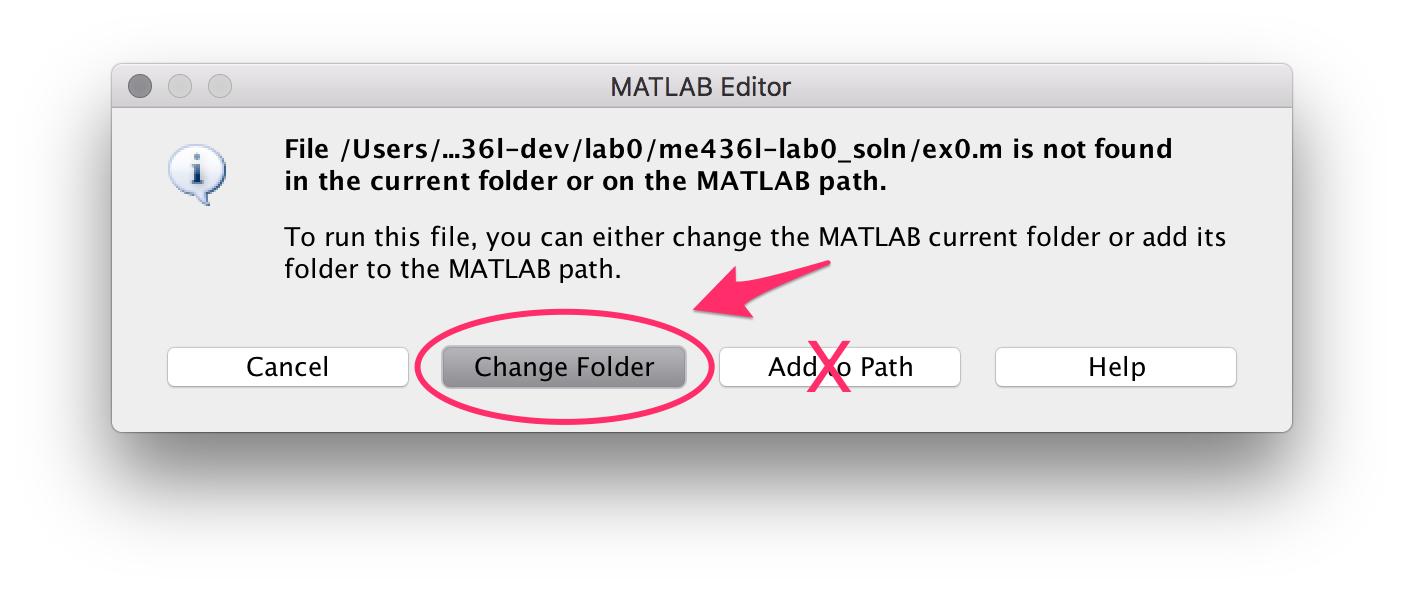
\includegraphics[width=100mm]{gfx/add_path_warning.png}
    \end{center}
\end{figure}

\item Remember, you cannot \textit{Run} a function by pressing the \texttt{`Run'} button. You can only do this for \textit{scripts}. See the Resources section below for more information.

\item \bul{Do NOT} use screenshots for reporting your results.
\begin{itemize}
    \setlength\itemsep{0.5em}
         \item \bit{Reason:} The default Matlab \textit{figure} window is designed for the screen, \textit{\ul{not print}}. This will turn out very small and blurry. 
         \item Simply do the following: \texttt{File >> Export Setup >> Apply to Figure >> Export >> Choose PNG Format.}
\end{itemize}


\end{itemize}


\newpage
\section*{Resources}
This section provides a list of helpful resources for getting started with Matlab. As always, your TA and classmates will be valuable resources as well.



\begin{itemize}
    \setlength\itemsep{0.5em}    

    \item \href{https://www.mathworks.com/help/matlab/getting-started-with-matlab.html}{Mathworks.com}: Here is a variety of resources produced by Mathworks. This covers the basics of Matlab, including a getting started tutorial.

    \item  \href{https://weblogin.iastate.edu/cgi-bin/index.cgi}{Lynda.com}: A video-based learning platform for a variety of topics. Normally this is a paid service, but ISU provides free access. To use this resource, do the following:

\begin{itemize}
    \setlength\itemsep{0.5em}
    \item \href{http://www.iastate.edu}{iastate.edu} \texttt{ >> Sign Ons >> More Sign Ons... >>}
    \item Then click the \href{https://weblogin.iastate.edu/cgi-bin/index.cgi}{Lynda.com} button.
    \item Once you fill in your credentials, type \texttt{MATLAB} into the search bar and select \textit{`Learning Matlab'}
    \item Here you will find a selections of 2-3min videos explaining specific aspects of Matlab.
\end{itemize}

\item \href{https://www.youtube.com/watch?v=wqxwIk3vzkI&list=PL7CAABC40B2825C8B}{Getting Started with Matlab}: A youtube playlist produced by Mathworks.

\item \href{https://www.youtube.com/watch?v=IoiB16fg3tQ}{What is Matlab and Why is it Used?} - A corny video explaining what Matlab is commonly used for.

\end{itemize}

\vspace{10mm}
\begin{itemize}
\item \bul{Finally, Ask questions!} It doesn't take much to e-mail your TA! If you don't ask, we cannot help!
\end{itemize}







\end{document}
